\chapter{Infrastruktur}
\label{infrastruktur}
\section{Server in der Cloud mit Amazon EC2}
Die Prämisse war von Anfang an klar: möglichst alle Dienste welche wir für diese Studienarbeit brauchen, sollen aus der \emph{\gls{Cloud}} kommen. Da liegt es natürlich Nahe, dies auch auf die Infrastruktur anzuwenden. Dank dem Amazon Free Usage Tier\footnote{\url{http://aws.amazon.com/free/}} konnten wir kostenlos Server bei Amazon EC2 aufsetzen.

Gemäss dem \gls{Cloud}-Ansatz, sind Ressourcen relativ kostengünstig, weshalb wir für jede Aufgabe einen separaten Server verwendet haben. So haben wir auch die Kopplung reduziert und können einzelne Dienste sehr einfach austauschen.

Insgesamt haben wir 3 Server verwendet:
\begin{itemize}
\item Build- und Deploymentserver: Build und Hosting der Sourcen
\item PhantomJS-Server: Ausführung der JavaScript-Tests 
\item Redmine-Server: Hosting der Projektmanagement-Software
\end{itemize}

Den Build- und Deploymentserver und den PhantomJS-Server haben wir selbst aufgesetzt. Den Redmine-Server mussten wir lediglich konfigurieren. Dies weil wir dafür auf einem bestehenden Image aufsetzen konnten, auf welchem Redmine schon installiert war. Das Open-Source Projekt BitNami\footnote{\url{http://bitnami.org/}} erstellt für zahlreiche Projekte solche Images. Dadurch entfällt ein Grossteil des Installationsaufwandes.

\section{Unit-Testing mit PhantomJS und QUnit}
Da wir hauptsächlich JavaScript als Programmiersprache verwendet haben, stellte sich bald einmal die Frage, wie sich unser Code sinnvoll testen lässt. Da wir bereits aus einem anderen Projekt sehr gute Erfahrungen mit QUnit\footnote{QUnit ist ein Unit Testing Framework von jQuery: \url{http://docs.jquery.com/QUnit}} gesammelt haben, wollten wir darauf aufbauen und haben damit unseren Code geprüft.

Da es sich auch bei unserem Testcode um JavaScript handelt, sind wir immer auf einen Browser angewiesen, welcher entsprechend die Tests ausführt. Für einen automatisierten Build ist dies unzureichend, da dieser nicht direkt die Tests ausführen kann.

Nach einigem Suchen sind wir schliesslich auf das Projekt PhantomJS\footnote{\url{http://phantomjs.org/}} aufmerksam geworden. Dabei handelt es sich um einen \gls{HeadlessBrowser}, welcher ohne grafische Darstellung auskommt. Damit konnten wir dann die URL unserer Tests\footnote{\url{http://gft.rdmr.ch/test/js/}} ansteuern und das Resultat in Jenkins auswerten\footnote{\url{http://phantomjs.rdmr.ch/gftprototype.php}}.

Es hat sich dann noch als Schwierigkeit ergeben, dass wir den Output von QUnit in eine für Jenkins verständliche Form bringen mussten. Dazu haben wir den Testrunner \inlinecode{run\_qunit.js} erweitert und mit zusätzlichen Ausgabemöglichkeiten ausgestattet. Alle nötigen Schritte haben wir schliesslich als Anleitung in einem Blogpost\footnote{\url{http://www.readmore.ch/post/18940470535}} veröffentlicht. Wir haben auch schon Feedback\footnote{\url{https://github.com/odi86/GFTPrototype/issues/1}} dazu erhalten und konnten so unsere Lösung weiter verbessern.

\section{Continuous Integration mit dem Jenkins Build-Server}
\label{build-server}
Bei Jenkins CI\footnote{\url{http://jenkins-ci.org/}} handelt es sich um ein Open Source Projekt, welches Unterstützung bietet für die Projektautomatisierung. Es unterstützt zahlreiche Repositories und Build-Mechanismen. Wir haben auch einige Plugins aktiviert, u.a. die GitHub- und Redmine-Integration oder der Logfile-Parser.

\subsection{Logfile-Analyse mit dem Log Parser Plugin}
Das Log Parser Plugin\footnote{\url{http://wiki.hudson-ci.org/display/HUDSON/Log+Parser+Plugin}} ermöglicht es auf einfache Art und Weise Probleme mit dem Build festzustellen. Für den Build kann es zum Teil sehr schwierig sein, den Status des Builds zu bestimmen. Der Build kann erkennen ob ein aufgerufener Befehl fehlgeschlagen hat oder ob die ausgeführten Tests erfolgreich durchlaufen. Wenn jedoch ein aufgerufenes Programm eine Warnung oder einen Fehler anzeigt, kann der Build das nicht selbst erkennen. Hier kommt der Logparser ins Spiel. Man kann Muster definieren für Dinge die auf eine Warnung oder einen Fehler hindeuten. Diese Logik erlaubt es dem Build viel detailliertere Aussagen über die laufende Installation zu machen.

\begin{figure}[!ht]
	\centering
	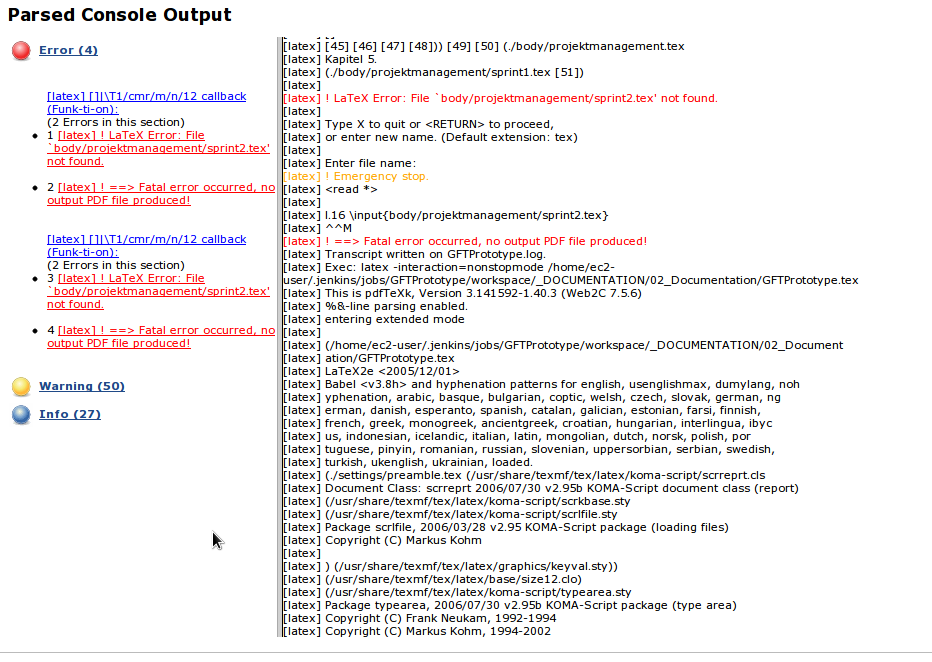
\includegraphics[width=\textwidth]{images/infrastruktur/jenkins-parsed-output}
	\caption{Ansicht des Logfiles mit dem Log Parser Plugin}
	\label{jenkins-parsed-output}
\end{figure}

\subsection{Trigger (Auslöser)}
Wir haben unseren Buildserver so getriggert, dass dieser ausgelöst wird, wenn eine Änderung auf GitHub gepusht wurde. Dazu haben wir das GitHub Plugin\footnote{\url{https://wiki.jenkins-ci.org/display/JENKINS/Github+Plugin}} auf Jenkins installiert, welches sich einfach im Backend installieren lässt. Im GitHub-Repository mussten wir dann noch sogenannte Web Hooks{\footnote{\url{http://help.github.com/post-receive-hooks/}} einrichten, so dass GitHub jeweils Jenkins benachrichtigt, sobald Änderungen eintreffen.

\subsection{Build Steuerung mit Ant}
Zur Build-Steuerung verwenden wir Ant\footnote{\url{http://ant.apache.org/}}. Ant ist vor allem aus der Java-Welt bekannt, lässt sich aber auch gut in andere Umgebungen einbinden. Der Build wir in einer \gls{XML}-Datei spezifiziert. Einzelne Schritte darin werden \emph{\gls{AntTarget}} genannt und diese sollten grundsätzlich von einander unabhängig sein. Dies ermöglicht es auch nur Teilschritte eines Builds auszuführen. Es lassen sich aber auch Abhängigkeiten zwischen Targets definieren, welche dann der Reihe nach abgearbeitet werden.

Hier zum Beispiel unser \inlinecode{build}-Target, welches alle anderen Targets als Abhängigkeit hat:
\lstset{language=Ant}
\begin{lstlisting}
<target name="build" depends="test,documentation,generate_css,deploy,test-js">
	<echo message="BUILD FINISHED!"/>
</target>
\end{lstlisting}

\subsection{Testausführung}
Zur Darstellung der Testresultate bauen wir auf dem JUnit \gls{XML}-Interpreter auf, welcher in Jenkins bereits integriert ist. Dazu ist es lediglich notwendig alle Testresultate in das JUnit \gls{XML}-Format zu bringen, die ganzen Auswertungen, Grafiken etc. bekommt man dann quasi "`gratis"' dazu.

\begin{figure}[!ht]
	\centering
	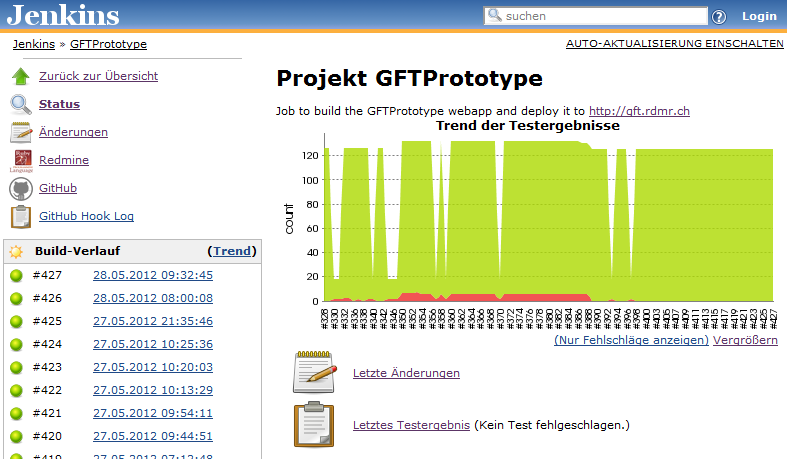
\includegraphics[width=0.8\textwidth]{images/infrastruktur/jenkins-test-results}
	\caption{Diagramm der Testresultate im Verlaufe der Zeit}
	\label{jenkins-test-results}
\end{figure}
